\documentclass[../main.tex]{subfiles}

\begin{document}
\section{Independent Observations (0D fields)}


\subsection{Univariate Observations}
Playfair bar graph, line graph, etc \cite{TufteVisualDisplay}
%%histogram and pdfs/distribution fitting

The specific shape is
dependent on what sort of density estimation method is used, such as kernal
estimation or nearest neighbor estimation \cite{chambers1983}. 
width using the density-trace method-which is a probability density estimation
via moving windowed average) proposed by Chambers et. al \cite{chambers1983},.


\subsection{Bivariate Observations}
\subsection{Multivariate Observations}
While bar graphs and histograms start giving a sense of the variability in
data, they are limited to showing the dispersion of the data only in 1
dimension; namely the measurements themselves. In their survey of the history
of the boxplot \cite{wickham2011} Wickham and Stryjewski trace the evolution of
the boxplot from a difinitive box to amorphous envelopes.  They start by laying
out
the core statistics of a boxplot, which can also be seen in
Figure~\ref{fig:boxplot}.
\begin{description}
\item[Median (Q2)] 50\% quartile
\item[Inter Quartile Range (IQR)]
\end{description}

\begin{tabular}{|r| r |r|r|}
  & Lower & Upper\\
  \multicolumn{2}{Hinge} & Q1: 25\%  & Q3: 75\% \\
  \multicolumn{2}{Interquartile range} & \multicolumn{2}{IQR = Q3-Q1}\\
  \multirow{2}{Fence} & Inner & Q1-1.5*IQR & Q3-1.5*IQR \\
  & outer & Q1-3*IQR & Q3+3*IQR \\
  \end{tabular}

\begin{figure}
  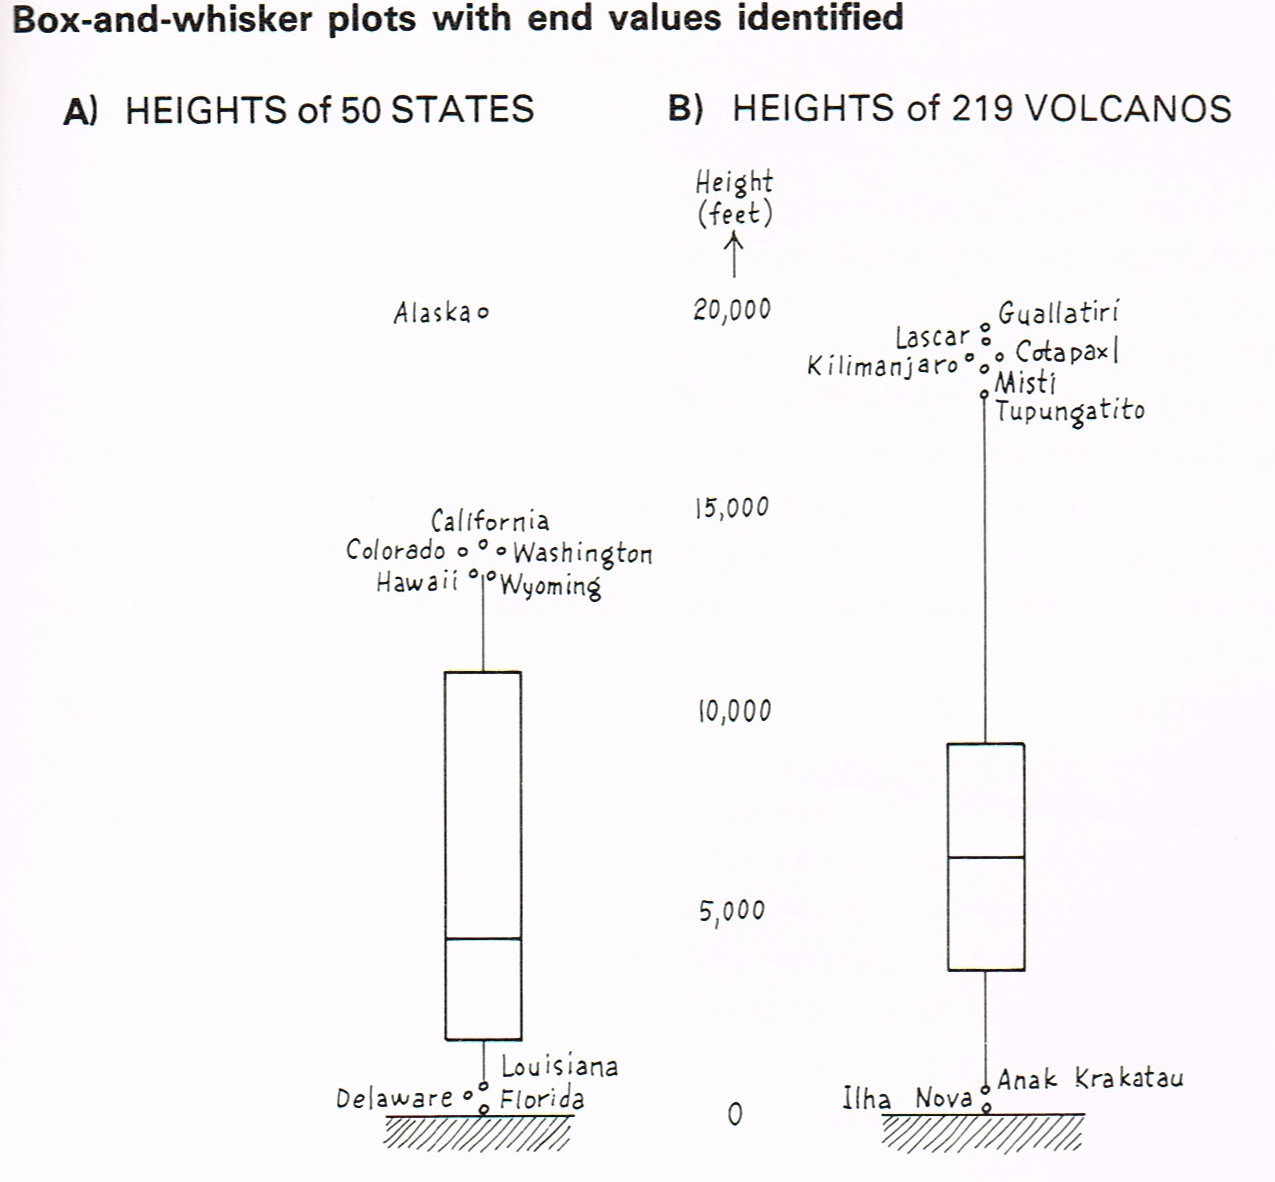
\includegraphics{boxplot}
  \caption{Tukey's 1977 example of the box plot (exhibit 6 of chapter 2 from
    Exploratory Data Analytics\cite{tukey1977}) illustrates how the box plot
    shows
    the distribution of topology of states and
    the distribution of volcanos. The strength of the box and whisker is that
    the
    reader can quickly compare the two distributions and learn, for example,
    that
    volcanos tend to span a shorter range of average heights, but that the
    extremes
    are much further from the center. Essentially, the distributions act as
    references for the other displayed distributions.}
  \label{fig:boxplot}
\end{figure}

In Tukey's introduction to the boxplot \cite{tukey1977}, shown in
Figure~\ref{fig:boxplot}, the box and whisker plot takes the distributional
information of a h\
istogram and encodes the state heights between the
25th and 75th percentiles as a box, the median height as a line cutting across
the heights, and the extreme state heights as lines coming out of the
boxes. While a histogram would also show that the distribution of state heights
has a fat righ\
t tail,
the power of the box and whisker plot is in encoding this information such that
it's trivial to compare to it's neighboring distribution of volcano
heights because they can share the Y axis. As the number of distributions grow,
this technique becomes invaluable because the number of histograms that can be
placed next to each other or overlayed as pdfs can quickly become
unweildy.  Many others authors have kept the basic structure of the boxplot,
but exploited the structure to convey more information about the data. Authors
used different quantile levels \cite{hyndman1996}s or measures of outliers
\cite{frigge1989}, or ways of identifying outliers\cite{carter2009,
  schwertman2004, schwertman\
  2007}, or otherwise incorporated skewness,
kurtosis, and other descriptive distributional statistics \cite{kim2004,
  hubert2008, marmolejo\
  2015}.

\begin{figure}
  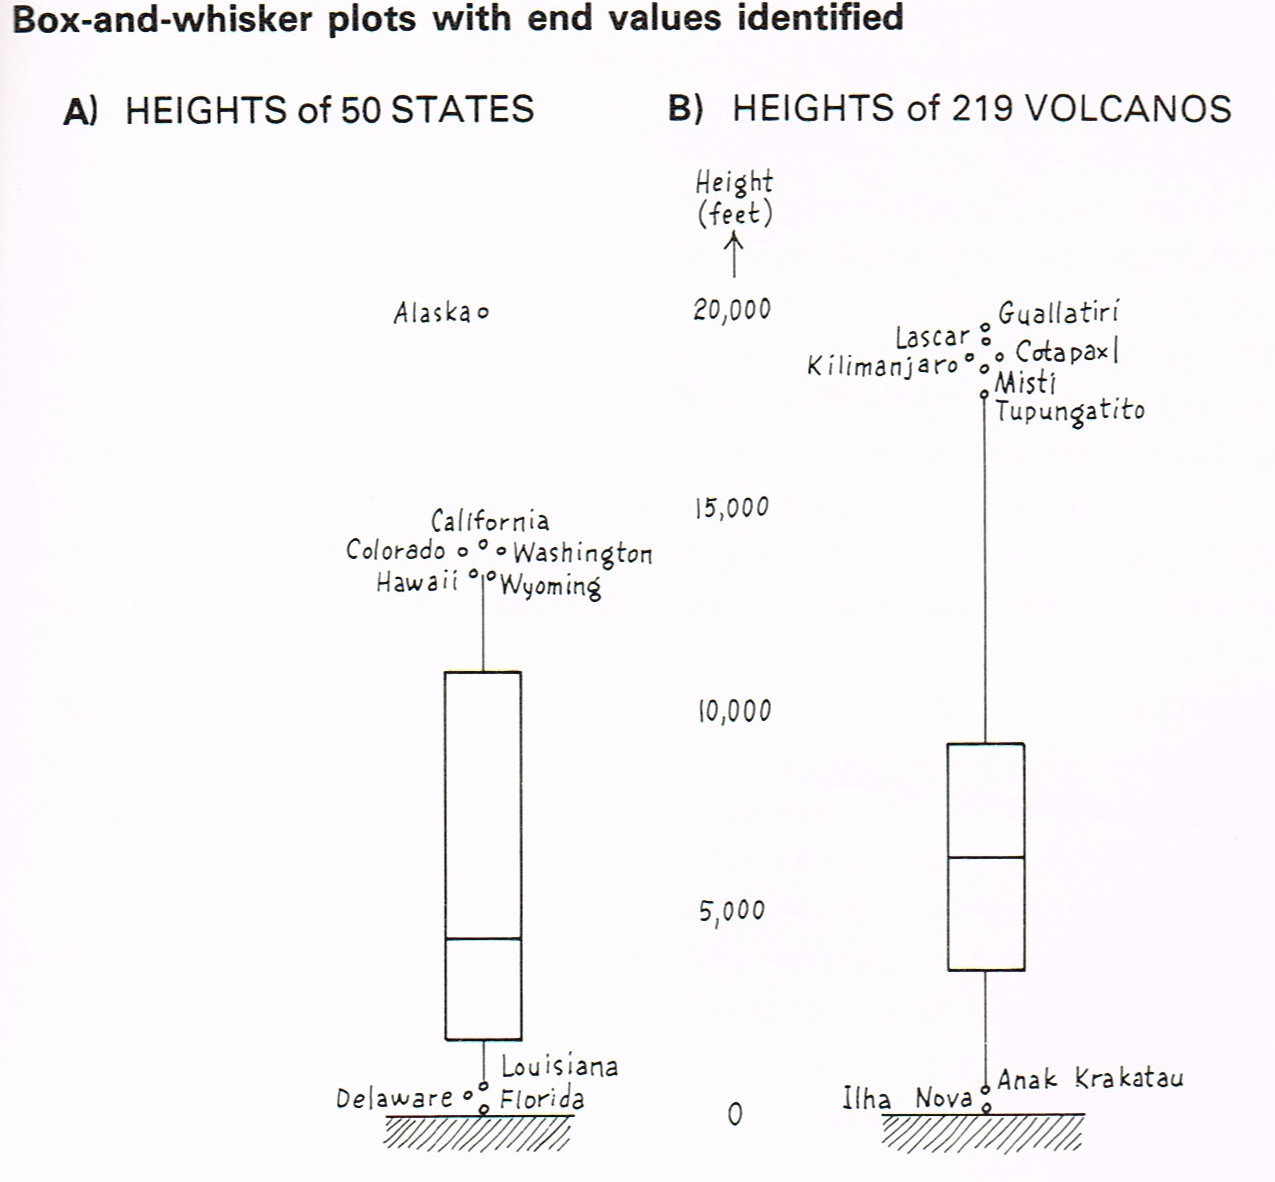
\includegraphics{boxplot}
  \caption{Tukey's 1977 example of the box plot (exhibit 6 of chapter 2 from
    Exploratory Data Analytics\cite{tukey1977}) illustrates how the box plot
    shows
    the distribution of topology of states and
    the distribution of volcanos. The strength of the box and whisker is that
    the
    reader can quickly compare the two distributions and learn, for example,
    that
    volcanos tend to span a shorter range of average heights, but that the
    extremes
    are much further from the center. Essentially, the distributions act as
    references for the other displayed distributions.}
  \label{fig:boxplot}
\end{figure}

In Tukey's introduction to the boxplot \cite{tukey1977}, shown in
Figure~\ref{fig:boxplot}, the box and whisker plot takes the distributional
information of a h\
istogram and encodes the state heights between the
25th and 75th percentiles as a box, the median height as a line cutting across
the heights, and the extreme state heights as lines coming out of the
boxes. While a histogram would also show that the distribution of state heights
has a fat righ\
t tail,
the power of the box and whisker plot is in encoding this information such that
it's trivial to compare to it's neighboring distribution of volcano
heights because they can share the Y axis. As the number of distributions grow,
this technique becomes invaluable because the number of histograms that can be
placed next to each other or overlayed as pdfs can quickly become
unweildy.  Many others authors have kept the basic structure of the boxplot,
but exploited the structure to convey more information about the data. Authors
used different quantile levels \cite{hyndman1996}s or measures of outliers
\cite{frigge1989}, or ways of identifying outliers\cite{carter2009,
  schwertman2004, schwertman\
  2007}, or otherwise incorporated skewness,
kurtosis, and other descriptive distributional statistics \cite{kim2004,
  hubert2008, marmolejo\
  2015}.

\subsection{Multivariate Observations}
%% large scale box: letter, spark


\subsection{Relationships Between Variables}
\subsubsection{Bivariate}
%%scatter segue into bagplot and HDR?
\begin{figure}
  %%\includegraphics{bagplot}
\end{figure}
The boxplot is inherently limited to 1D data; the bagplot was introduced to
visualize 2D and higher data \cite{rousseeuw1999}
Bivariate HDR plot \cite{hyndman1996} \textbf{expand with discussion of
  boxplot/HDR plot}

\subsection{Multivariate Observations}

%% radial, parallel coordinates, factor plotl
%%high d-PCA, ICA, markov


